\chapter{Thermal Phase Curves}
\label{thermalphasecurves}
Although transits are useful, particularly for determining atmospheric species,
 they tell little about how the surface of a
 planet may look. Transits can only see the terminator profile, and would
 therefore only see a small section of the total atmosphere. In order to push
 our understanding of exoplanets, we would ideally like a method to measure an
 atmosphere across the planet instead of in a thin terminator. With this goal
 in mind, measuring the thermal emission of an exoplanet directly sounds like
 a promising technique. The most reliable way of doing this is by measuring the
 change
 in the thermal emission over time. For all transiting exoplanets, their
 surface will rotate relative to an observer. In Chapter \ref{models}, we
 found that there was significant structure to the atmosphere as well as
 significant variability over longitude. Therefore, thermal phase curves
 merit serious consideration as an observational technique for probing
 exoplanetary atmospheres.

In order to examine an exoplanetary atmosphere's thermal emission, we must first
 chose which wavelengths to examine. To first order, assuming that the host star
 and exoplanet emit as a blackbody, the ratio between the thermal emission of
 the two will always increase towards longer wavelengths. This can be confirmed
 by using the PSG. Using a global disk average for each phase, in increments of
 $5\deg$, the PSG can be run, producing different signals at different points in an exoplanet's year. Some wavelengths do not experience strong temporal
 variability over time. To determine which wavelengths produce strong signals,
 we can compute $F_\mathrm{max}-F_\mathrm{min}$, which is shown in Figure
 \ref{tpc_max_diff}. Longer wavelengths will change dramatically across phase,
 up to $80\,\mathrm{ppm}$, while shorter wavelengths will change very little
 because the light in the shorter wavelengths is dominated by the host star.
 The longest wavelengths vary more dramatically than the transit spectra with
 and without species in Figure \ref{nospecies}. The variability in thermal emission
 changes dramatically, even between individual wavelengths. This is due to the
 molecular behavior of atmospheric species across different temperatures,
 primarily \chem{H_2O}.

 \begin{figure}[ht]
    \begin{center}
        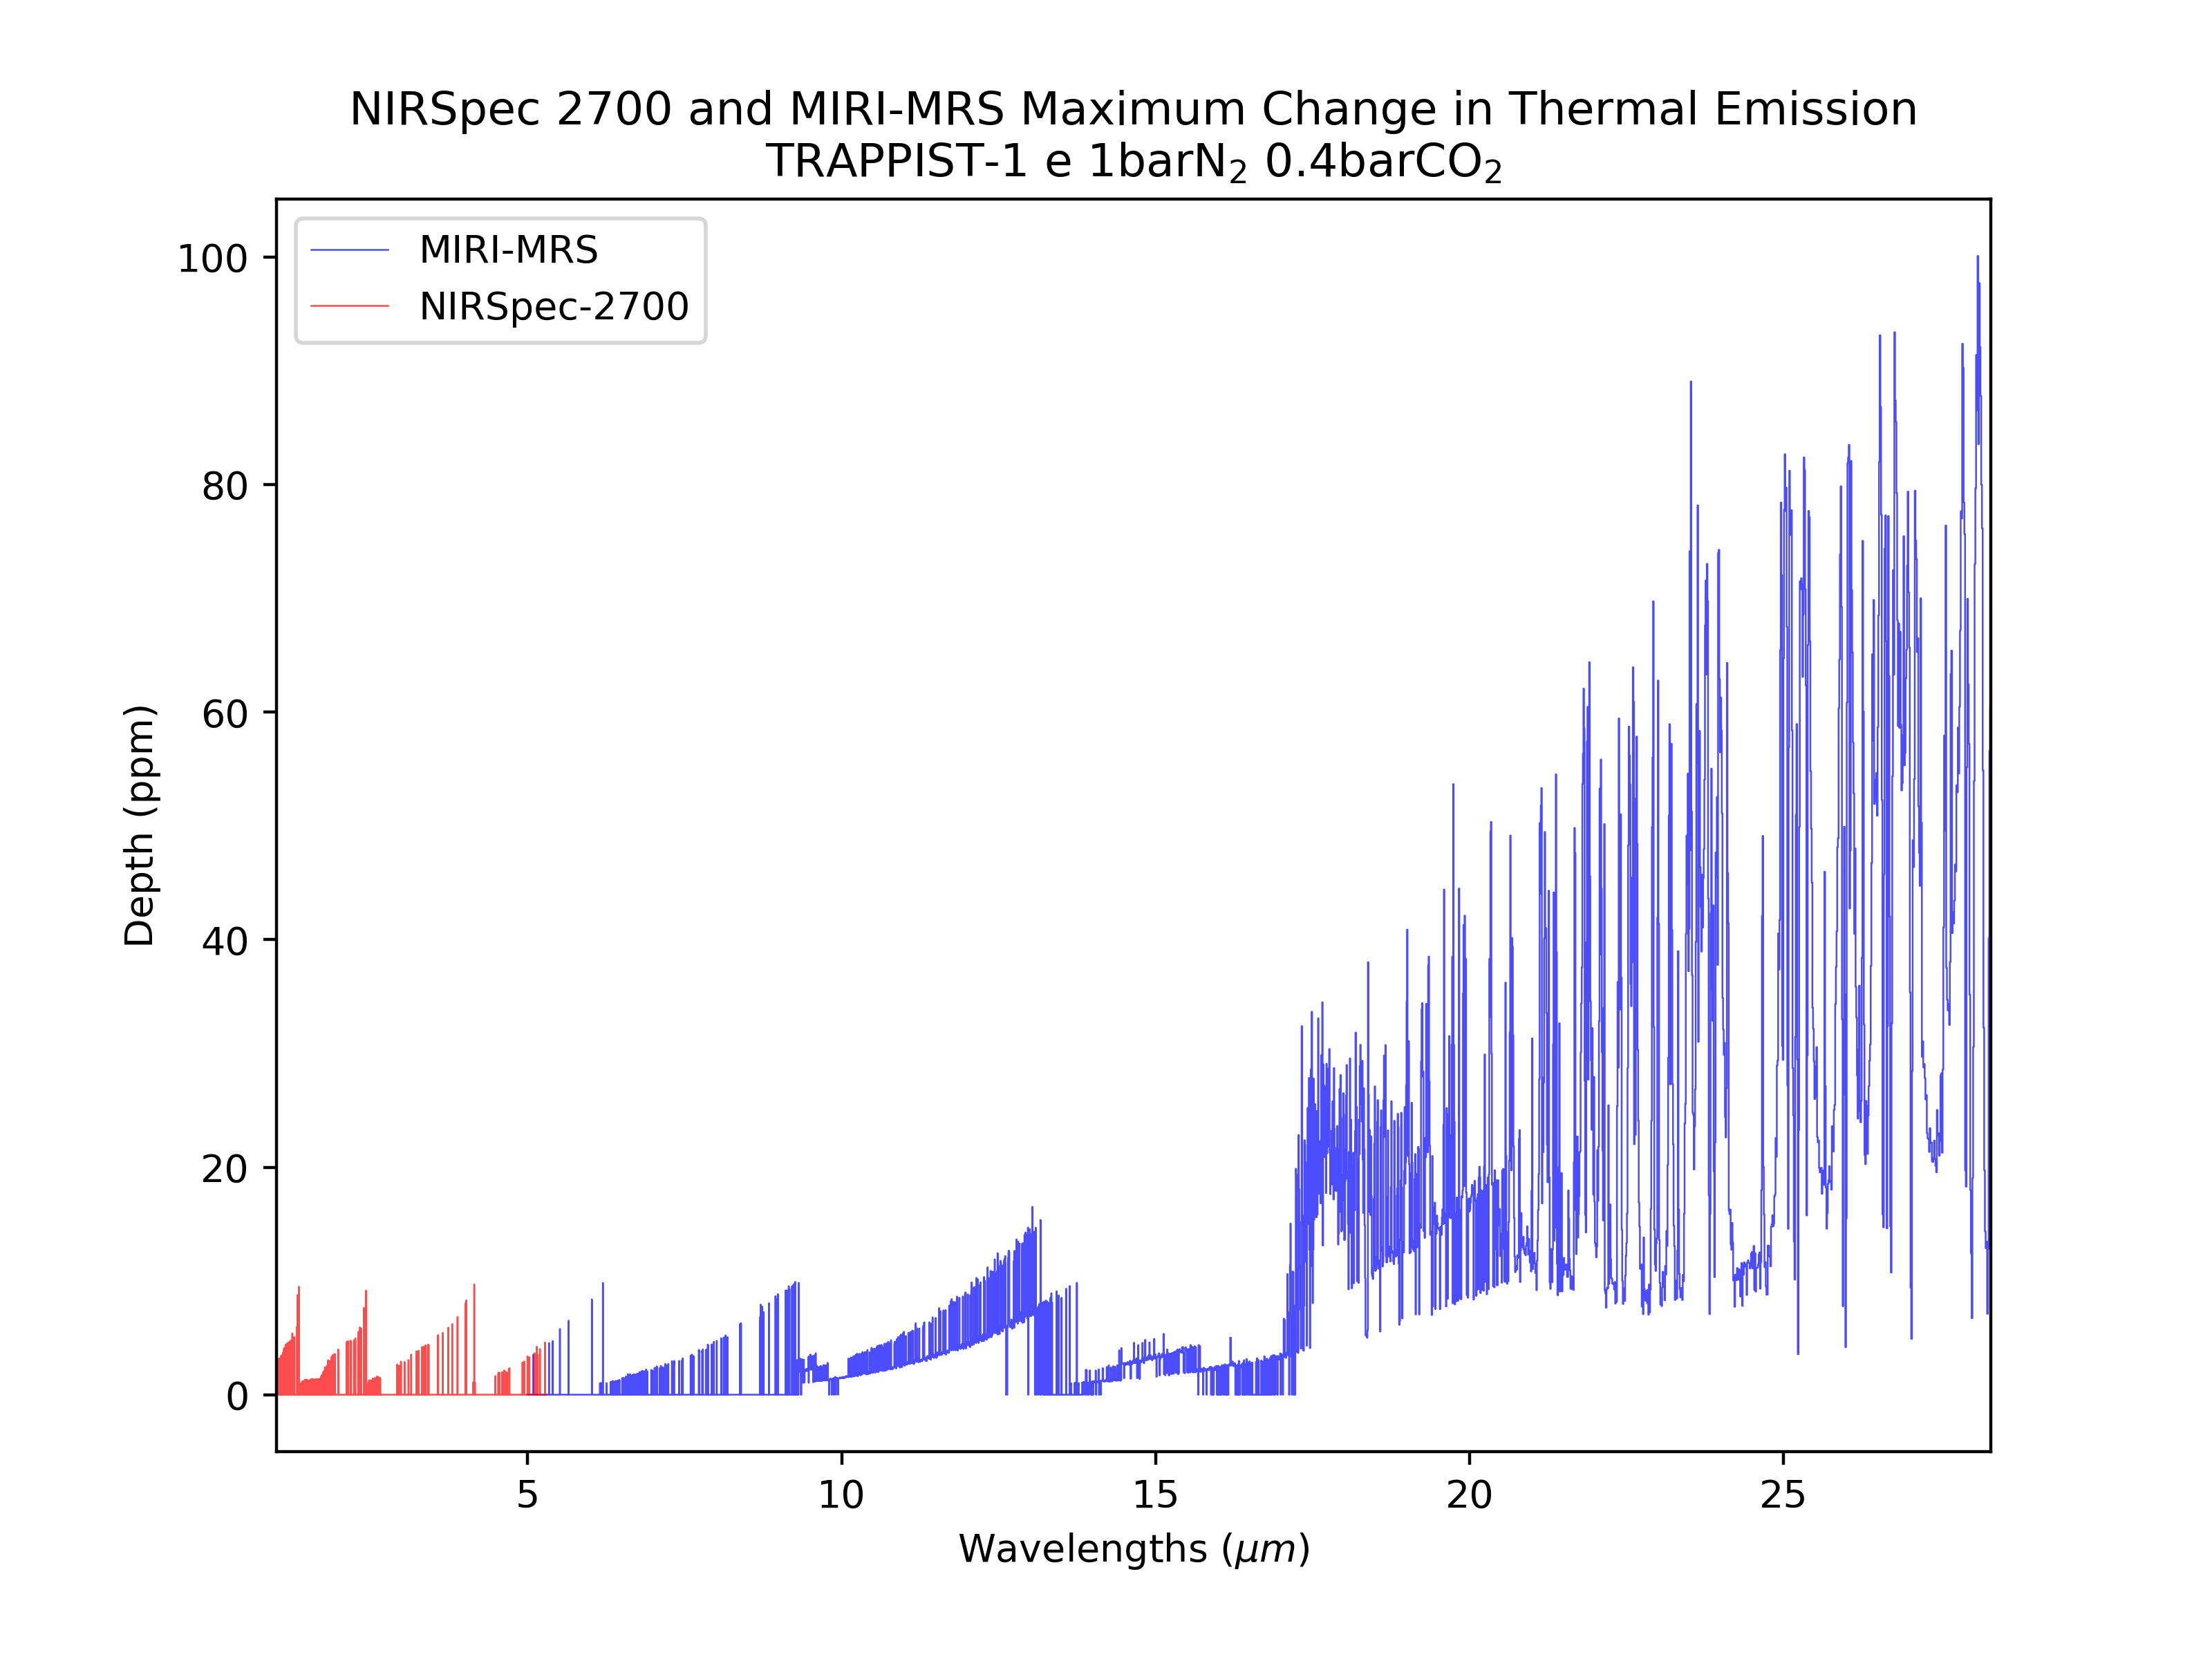
\includegraphics[width=\textwidth]{tpc/tpc_max_diff.png}
        \caption[Maximum Change of Thermal Emission Over Time]{Maximum Change of
        Thermal Emission Over Time. NIRSpec and MIRI are shown together, and
        the y axis is the maximum thermal emission minus the minimum thermal
        emission. This technique demonstrates that longer wavelengths
        will experience stronger variability in thermal emission over time.}
        \label{tpc_max_diff}
    \end{center}
\end{figure}

According to Figure \ref{tpc_max_diff}, the most optimal wavelengths for thermal
 phase curve analysis are longer wavelengths, primarily to the right of the
 $\SI{17}{\micro\meter}$ jump, although wavelengths as short as $\SI{10}{\micro\meter}$ should be considered in
 the interest of reducing noise, although it would also reduce the magnitude of
 the signal by including lower values. Similar to transits, a subset of
 wavelengths can be defined such that

\begin{equation}
    \frac{F_\mathrm{max}(\lambda)-F_\mathrm{min}(\lambda)}{F_*}(\lambda)
    \geq 8\,\mathrm{ppm},
\end{equation}
but this will not prove as useful here as it did for transits because a number
 of these features in Figure \ref{tpc_max_diff} are extremely thin, and so
 reliably binning those values is impractical. In this case,
 $\lambda\geq\SI{17}{\micro\meter}$
 will prove to be the most reliable method because of its simplicity, while other
 techniques don't provide much advantage for their added complexity.

 \begin{figure}[ht]
    \begin{center}
        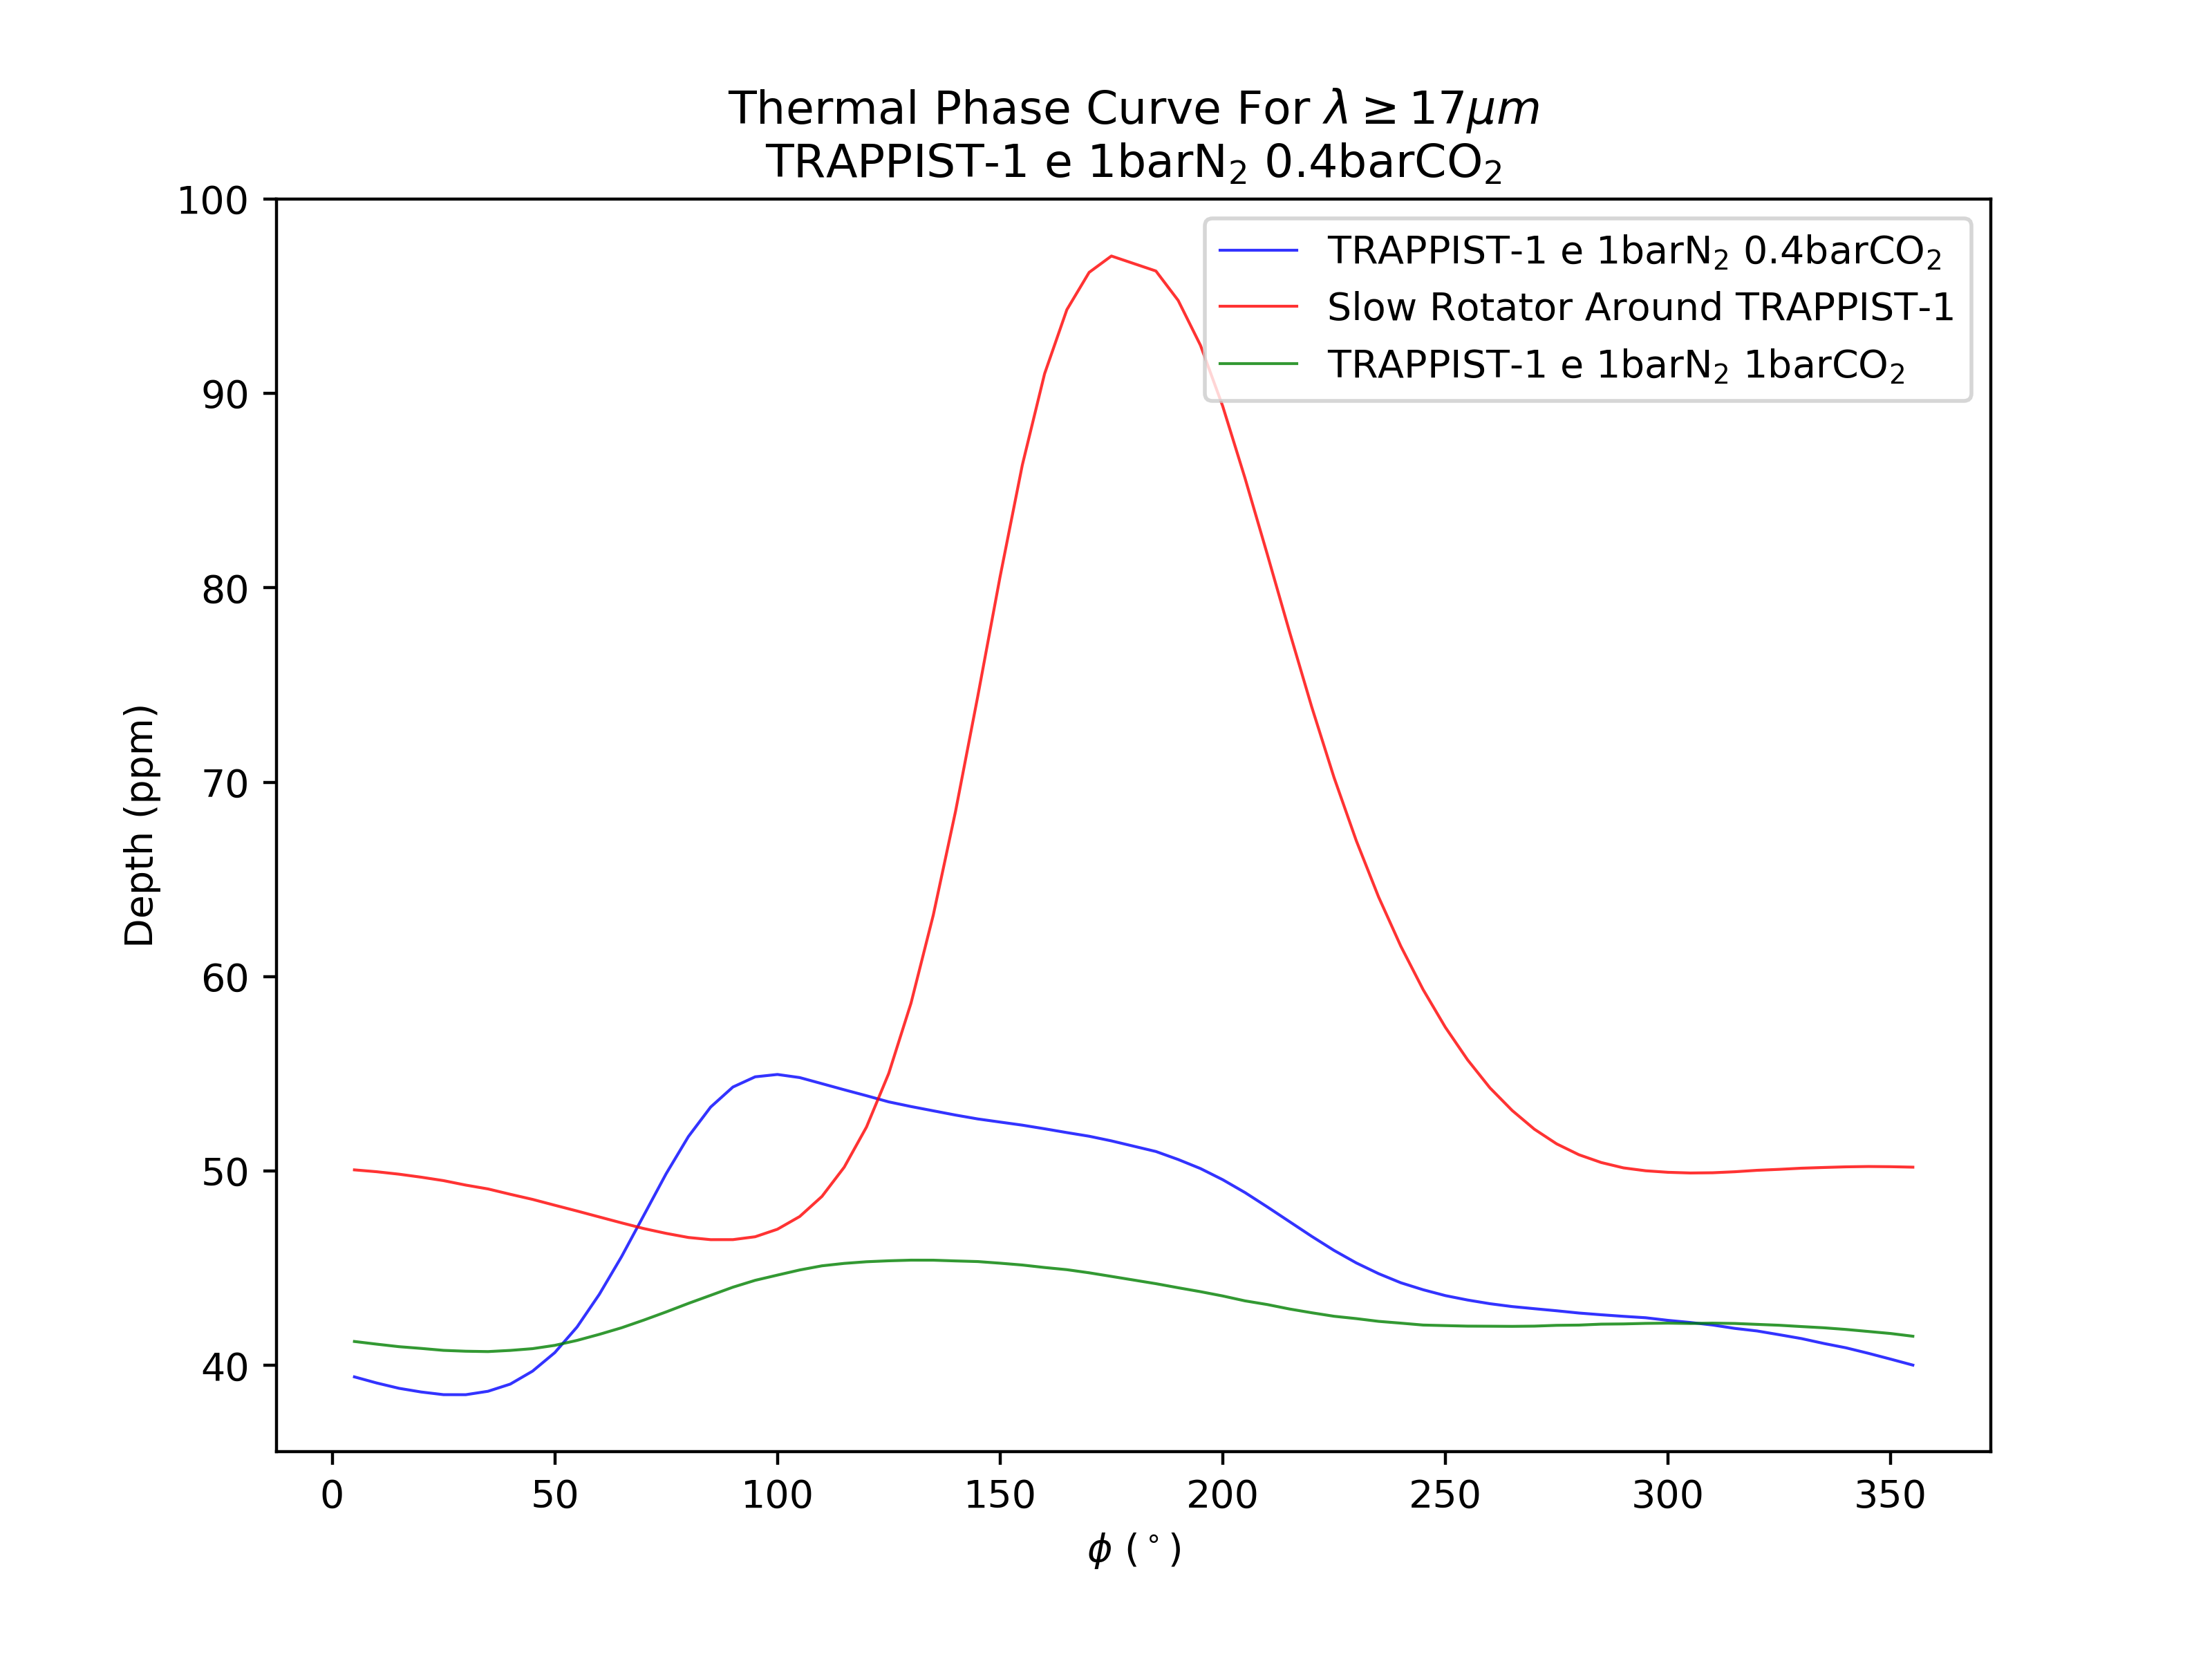
\includegraphics[width=\textwidth]{tpc/thermal_phase_curve.png}
        \caption[Thermal Phase Curve of TRAPPIST-1 e]{Thermal Phase Curve of
        TRAPPIST-1 e. The x axis here is orbital phase, but this value is
        linearly correlated with time. $\SI{0}{\degree}$ is correlated with an
        occultation and $\SI{180}{\degree}$ is correlated with a transit. 
        However, both of those points were excluded from the plotted results
        because those values were
        discontinuous with the trend. The steep climb is from when the
        cloud-free areas rotate out of view toward Earth, and the gradual decline
        is where
        the night side rotates out of view, and eventually bottoms out when the
        substellar cloud is in view. Even if these features about the surface
        weren't known, this data could be used to infer the distribution of
        clouds on the surface. The red case, using the same climate model from 
        Figure \ref{slowrotator} is highly symmetric because the cloud distribution
        is highly symmetric. The hot case with $\SI{1}{\bar}$ \chem{N_2}
        $\SI{1}{\bar}$ \chem{CO_2}
        is so low because there are little to no clouds like in the temperate
        case, so the thermal phase curve is virtually flat. If shorter
        wavelengths than $\SI{17}{\micro\meter}$ were included in this, they
        would produce the same shape, but the overall thermal phase curve will
        be over a smaller magnitude.}
        \label{tpc}
    \end{center}
\end{figure}

In a thermal phase curve like the one shown in Figure \ref{tpc}, the shape is
 roughly the same across all wavelengths of any fixed climate model, and the
 phase of the steepest slope is highly dependent on which model is being
 simulated. The magnitude of this jump is dependent
 on the wavelength range examined. Including more wavelengths in the summation
 will improve signal to noise, but reduce the magnitude of the jump. The longest
 wavelengths produce the strongest jumps, but they also have the largest noise.
 Unlike transit spectra, where the different models would only produce mildly
 different results, a thermal phase curve produces varied results across models.

The most exciting result from Figure \ref{tpc} is that the most habitable model
 of $\SI{1}{\bar}$ \chem{N_2} $\SI{0.4}{\bar}$ \chem{CO_2} stands out distinctly from
 the other models
 both in the location of its steep rise and the shape of its gradual decline.
 This suggests that thermal phase curves would be the most likely technique to
 distinguish between a habitable exoplanet with a stable atmosphere and an
 uninhabitable exoplanet.

Unfortunately, thermal phase curves using spectrographs on JWST are plagued with
 noise, the results shown in Figure \ref{tpc} produced a noise of 407ppm,
 which far outweighs any signal. However, this technique isn't optimized for
 spectroscopy. For transits, it is advantageous to use spectroscopy as it can
 identify many interesting emission features from different molecular species,
 but in this case, there are no specific features to identify, so there is
 no disadvantage to using a long-wavelength filter and a CCD. MIRI also has an
 imaging instrument on it, with two filters that would be useful for
 this purpose, F2100W and F2550W, but the F2550W filter is the most obvious
 candidate because it operates at the longest wavelengths JWST can probe.
 Although the PSG is a tool designed primarily for the purposes of simulating
 spectrograph, a high resolution spectra is still useful for predicting
 broadband photometry measurements as photometry depends on the filters used
 and therefore the wavelengths probed.